\documentclass[a4paper,10pt]{article}
\usepackage[english]{babel}
\usepackage[utf8]{inputenc}
\usepackage{graphicx}
\usepackage{multirow}
\usepackage{hyperref}
\usepackage{listings}
\usepackage{xcolor}
%Includes "References" in the table of contents
\usepackage[nottoc]{tocbibind}
\usepackage[nottoc]{tocbibind}
\lstdefinestyle{customc}{
    belowcaptionskip=1\baselineskip,
    breaklines=true,
    frame=L,
    xleftmargin=\parindent,
    language=C,
    showstringspaces=false,
    basicstyle=\footnotesize\ttfamily,
    keywordstyle=\bfseries\color{green!40!black},
    commentstyle=\itshape\color{purple!40!black},
    identifierstyle=\color{blue},
    stringstyle=\color{orange},
}

\lstdefinestyle{customasm}{
    belowcaptionskip=1\baselineskip,
    frame=L,
    xleftmargin=\parindent,
    language=[x86masm]Assembler,
    basicstyle=\footnotesize\ttfamily,
    commentstyle=\itshape\color{purple!40!black},
}

\lstset{escapechar=@,style=customc}
%Title, date an author of the document
\title{An Analysis of Oil / Oil Products Relationships in Different Markets}
\author{Promo Anene: promo.anene@yahoo.com \\
        Ruphin Aganze: jfrayruphin@yahoo.fr \\
        Tarun Kumar: bing.tome@yahoo.co.in \\}


%Begining of the document
\begin{document}

\maketitle

\medskip
\begin{abstract}
    \it{Crude oil is a key commodity in world economy. It finds strategic importance and varied uses in many diverse applications, industrial and domestic. These include transportation, industrial power, home energy and everyday products such as plastics, drugs etc. In combination with other chemicals, oil forms the base of over thousands of products.


    Crude oil is also a highly volatile asset that is subject to wide price swings. In the world of financial engineering, it is not uncommon to find portfolios comprising assets that are directly or indirectly linked to crude oil or its products.


    In order to maximize gains from oil-related assets, it is necessary to understand its price drivers. In this regard, it is noteworthy that crude oil prices are driven primarily by the price of its refined products. These include gasoline, diesel, jet fuel, naphtha, fuel oils etc. This research project investigates the price relationship between crude oil and its refined products for different crude blends defined by geographical locations (WTI, Brent and Bonny Light). Statistical analysis is conducted on 20-year price data. The analysis primarily comprises time series analysis of spreads and tests for mean reversion and correlation across different time periods.

    We find that indeed, a price relationship exists between crude oil and its products to varying degrees for the blends tested (WTI, Brent and Bonny Light). We hope that this research work can enable predictions of short-term price changes for oil and product commodities. We also expect that the relationship established in this research work can be leveraged in portfolio risk management and portfolio diversification.}
\end{abstract}

\textbf{Keywords: crude oil, refined product, West Texas Intermediate, WTI, Brent, Bonny Light, equilibrium modelling.}
\section{Introduction}
Oil forms the lifeblood of the world’s economy. Oil products underpin modern society and are used in a wide range of industrial and domestic application. These include transport fuels, industry power, home heating and manufacture of everyday products such as plastics, medicines, detergents, paints etc. As a result, the prices of refined oil products play a key role in stabilizing world economy and social order.\newline

Oil prices are subject to wide price swings due to the forces of demand and supply i.e. it has experienced high prices occasioned by periods of high demand, but also depressed prices due to oversupply and low demand. These so-called price cycles tend to last several years, depending on variables such as oil demand, volume of oil drilled, processed and sold by major producers, including integrated oil companies (IOU's), geopolitical factors etc.

\begin{figure}[h]
    \centering
	\noindent\makebox[\textwidth]{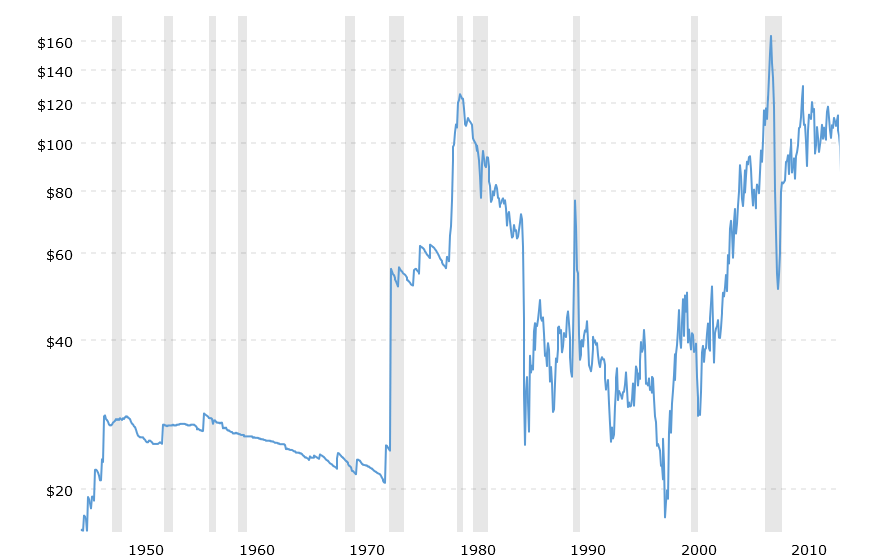
\includegraphics[width=0.6\paperwidth]{images/image1.png}}
	\caption[Oil Price]{Wide price swings in oil prices.\footnote{https://www.macrotrends.net/1369/crude-oil-price-history-chart}}
    \label{fig:oilprice1}
\end{figure}

Notwithstanding the price swings, crude oil is a widely traded and important commodity in the world. As earlier noted, it is a key underpinning factor in many economies. There is a well-established and highly competitive international market for this commodity. It is a sophisticated financial product with high uncertainty and volatility.\newline

The key factor that affects the price of oil products such as gasoline is the corresponding crude oil price. An effective understanding of the relationship between crude oil prices and their corresponding refined products, can enable predictions of short-term price changes. Also, and very importantly, the relationship between crude oil and refined products can be leveraged in portfolio risk management and portfolio diversification.\newline

Portfolio diversification is a risk management strategy where a variety of assets are combined in order to reduce overall risk of the investment portfolio. Effective asset combination in this regard requires that the asset mix are not highly inter-correlated. Otherwise, where asset co-variance is high, portfolio risk reduction due to diversification is reduced. It is thus important to investigate the relationship between crude and refined products to enable portfolio risk management especially with price variability for a portfolio of crude and refined products, such as for integrated oil companies which both produce and refine crude oil.\newline

This project will assess price relationships for crude oil and their refined product (gasoline et al) in three regions as follows:
      \begin{enumerate}
          \setlength{\itemindent}{.1in}
          \item The United States – US crudes vs. Western Texas Intermediate (WTI)
          \item Nigeria – Bonny Light crude vs. Nigerian Petrol prices
          \item North Sea crudes – Brent Blend vs. gasoline prices
      \end{enumerate}

	
The project will enable enhanced understanding of crude oil/refined products relationships and thus enhance effective portfolio risk management for crude and refined products portfolio mix, as well as asset price prediction for effective trading strategy.
The project objectives include:
    \begin{enumerate}
        \setlength{\itemindent}{.1in}
        \item Perform Exploratory Data Analysis on price data for crudes and products
        \item Compare key statistical metrics across the different markets
        \item Provide insights and possible economic explanations for the observed differences
    \end{enumerate}

\section{Theoretical Framework}
\subsection{Introduction}
There have previous research efforts into investigating the relationships between crude oil prices and their refined products counterparts. These researches have been mostly of a broad market review nature. One key research in this area is the work by Gjolberg and Johnsen (2003, Risk management in the oil industry: Can information on long-run equilibrium prices be utilized) \cite{joh99,gjo03} in which it is established that a long-term relationship does exist between crude and refined products.

There have also been other studies and efforts to model oil prices. The work by Fischer D., Gately D., Kyle J. (1975)\cite{fis75} is one of the early research studies conducted on oil price modelling.  The studies by Bacon and Kojima (2006 and 2008)\cite{bac06, bac08} was with an emphasis on statistics and economics. Many other studies, while reviewing oil price fluctuations do not specifically focus in-depth on the price relationship between crude oil and their corresponding refined products per blend.

Many studies also find that the transmission of positive and negative changes in crude prices to the refined products (gasoline et al) is asymmetric\cite{bor97, pol16}. Specifically, responses to price increases are much quicker than for price decreases. This is more evident in the US market than for the Euro region where mixed results have been noted.

In developing countries, refined product prices are more subject to price control constraints. A review carried out by the International Monetary Fund (IMF) found that out of 48 developing economies considered, only 16 countries have implemented a market-based pricing system for refined petroleum\cite{coa06}. In Nigeria, this is effected through a Federal Government fuel subsidy programme.

This literature review analyses the main work carried out by Gjolberg and Johnsen (2003, Risk management in the oil industry: Can information on long-run equilibrium prices be utilized)\cite{joh99} and establishes the additional contributions this research project will make to the already established body of knowledge in this regard.

\subsection{Review of Existing Literature}
This literature review will focus on the work by Gjolberg and Johnsen (2003, Risk management in the oil industry: Can information on long-run equilibrium prices be utilized)\cite{gjo03}. The work investigated price volatility and correlations between crude oil price and refined products (Premium gasoline, naphtha, jet fuel, gas oil light fuel oil and heavy fuel oil) between the periods from January 1992 to August 1998.

\subsection*{Data Source}
The data set was sourced from Platt’s. Monthly observations were used by picking the prices recorded on the 15th of each month or the closest day of business.
\begin{figure}[h]
    \centering
	\noindent\makebox[\textwidth]{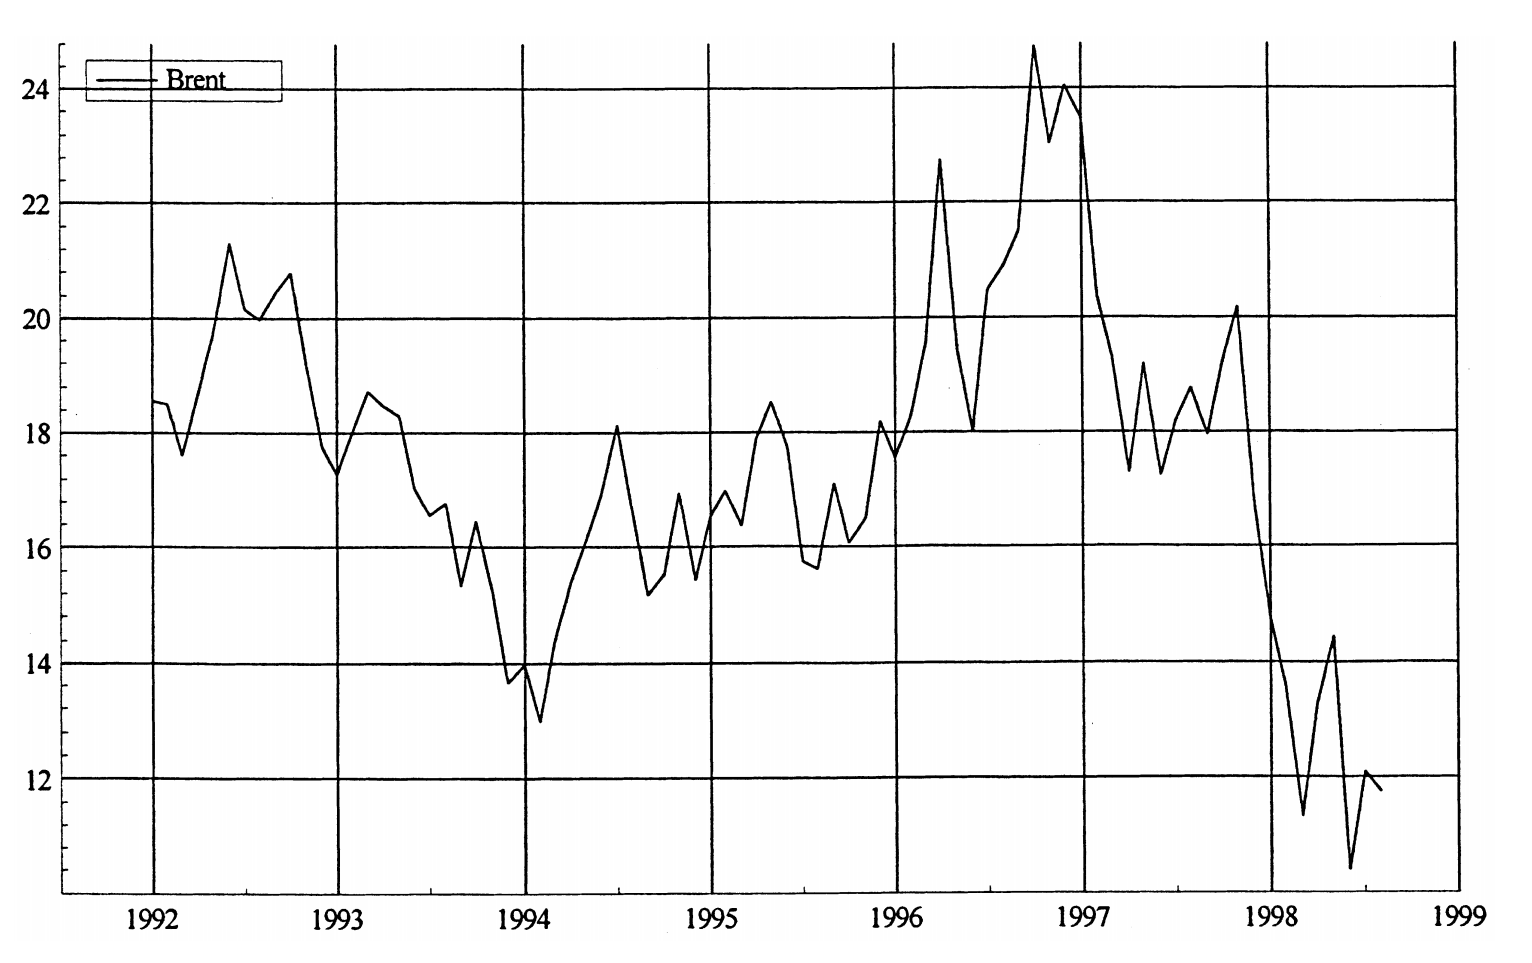
\includegraphics[width=0.4\paperwidth]{images/image2.png}}
	\caption[Oil Price]{Crude Brent price US \$ Ž. rbbl, January 1992] August 1998.}
    \label{fig:oilprice2}
\end{figure}

The data shows the wide variability of Brent prices within the period of study. High price volatility is observed, including a low of US\$13/bbl in 1994, a high of above US\$24/bbl in 1996 and a crash to US\$11/bbl in 1998.

\section*{Exploratory Analysis and Econometric Results}
Table 1 below shows the coefficients of price variations and the annualized standard deviation of monthly price changes (\%). As observed, the coefficients of variation do not differ much between crude oil (16.1) and the products – except for heavy fuel oil (21.9).

\begin{table}[h!]
\begin{tabular}{|p{3cm}|p{4cm}|p{4cm}|}
    \hline
    & Cofficient of variation, Price level (\%) & Annualized S. D. monthly percentage price change (\%)\\
    \hline
     Crude & 16.1 & 30 \\
     Premium Gasoline & 13.5 & 30 \\
     Naphtha & 14.4 & 26 \\
     Jet Fuel & 15.6 & 24 \\
     Gas Oil & 15.9 & 27 \\
     Light Fuel Oil & 16.3 & 39 \\
     Heavy Fuel Oil & 21.9 & 44 \\
     \hline
\end{tabular}
\caption{Price Volatility, 1992 - 1998}
\label{table:1}
\end{table}

\noindent The correlations for price level and price changes are shown below in Table 2 and Table 3 respectively:
\begin{table}[h!]
\begin{tabular}{|p{2.5cm}|p{1cm}|p{1.5cm}|p{1.5cm}|p{1cm}|p{1cm}|p{1cm}|}
    \hline
    & Crude & Premium gasolin & Naphtha & Jet Fuel & Gas Oil & Light Fuel Oil \\
    \hline
     Premium & 0.86 & & & & &\\
     Naphtha & 0.94 & 0.86 & & & &\\
     Jet Fuel & 0.92 & 0.74 & 0.84 & & &\\
     Gas Oil & 0.93 & 0.78 & 0.86 & 0.98 & &\\
     Light fuel Oil & 0.77 & 0.56 & 0.70 & 0.69 & 0.68 &\\
     Heavy fuel Oil & 0.67 & 0.40 & 0.63 & 0.56 & 0.55 & 0.88 \\
     \hline
\end{tabular}
\caption{Price level correlations, 1992 – 1998 (monthly observations)}
\label{table:2}
\end{table}

\begin{table}[h!]
\begin{tabular}{|p{2.5cm}|p{1cm}|p{1.5cm}|p{1.5cm}|p{1cm}|p{1cm}|p{1cm}|}
    \hline
    & Crude & Premium gasolin & Naphtha & Jet Fuel & Gas Oil & Light Fuel Oil \\
    \hline
     Premium & 0.62 & & & & &\\
     Naphtha & 0.72 & 0.65 & & & &\\
     Jet Fuel & 0.77 & 0.45 & 0.55 & & &\\
     Gas Oil & 0.78 & 0.56 & 0.59 & 0.89 & &\\
     Light fuel Oil & 0.47 & 0.34 & 0.39 & 0.44 & 0.43 &\\
     Heavy fuel Oil & 0.48 & 0.33 & 0.46 & 0.44 & 0.41 & 0.69 \\
     \hline
\end{tabular}
\caption{Price change correlations, 1992 – 1998 (monthly observations)}
\label{table:3}
\end{table}

As seen above, the co-changes between the price level for crude oil and the refined products is quite high – 86\% and 93\% for premium gasoline and gas oil. The figures are slightly lower for LFO and HFO at 77\% and 67\% respectively. Similarly, there is relatively high correlation between crude and products price changes. The correlations between crude and the heavier fuel oils are lower, as with the correlations between lighter products and the heavier ones. As earlier noted, these correlations represent valuable insight for portfolio diversification and risk management.

\noindent The main statistics from Ordinary Least Squares (OLS) estimation are shown below.

\begin{table}[ht]

\begin{tabular}{|c@{\qquad}cccc@{\qquad}ccc|}
  \hline
  \multicolumn{1}{|l}{} & \multicolumn{3}{l}{{Short run dynamic model}} & \multicolumn{1}{l}{}& \multicolumn{3}{l|}{{Solved long-run}} \\ 
  \cline{2-4}
  \cline{6-8}
  & $F_{7, 72}$ & DW & Adj.$R^{2}$& &$\beta_{1}$ & S.E. & Wald $\chi^{2}$ \\
  \hline
  Gasolin & $47.17^{**}$ & 1.97 & 0.82 & &0.76 &0.10 &$57.41^{**}$ \\
  Naphtha & $133.17^{**}$ & 1.98 & 0.93 & &0.96 & 0.07 & $190.57^{**}$ \\
  Jet fuel & $146.86^{**}$ & 1.98 & 0.93 & &0.97 & 0.11 & $78.94^{**}$ \\
  Gas oil & $132.66^{**}$ & 1.98 & 0.93 & &0.99 & 0.11 & $76.94^{**}$ \\
  Light fuel oil & $31.44^{*}$ & 1.93 & 0.75 & &0.54 & 0.16 & $11.40^{**}$ \\
  Heavy fuel oil & $46.93^{**}$ & 1.97 & 0.82 & &0.06 & 0.48 & 0.02\\
  \hline
\end{tabular}
\caption{– Summary of estimation results – OLS}
\label{tab:ols}
\end{table}

\noindent In table-\ref{tab:ols} above, the F-values are all significant at 1\% level. The Durbin-Watson statistics which measures auto-correlation are all close to 2.0 i.e. very low positive auto-correlation. The explained variance, as indicated by Adj. R2, range from 75\% for LFO to 93\% for naphtha, jet fuel and gas oil.

The research concludes by establishing that there is indeed a long-run spot price relationship between crude and refined products. In effect, for all refined products, possibly excluding heavy fuel oil, product prices are co-integrated with the crude price\cite{ben94}.
\subsection{Strengths and Opportunities of Current Research}
Current research has built on previous research works. To illustrate, previous research studies have tended to focus on the convergence of spot and future prices towards delivery (e.g. Ng and Pirrong, 1996)\cite{pir96} or the price discovery roles of futures vs. spot prices (e.g. Quan, 1992; Schwarz and Szakmary, 1994)\cite{qua92}. The work by O. Gjolberg and T. Johnsen (1999) instead drew attention “to the long-run spot price relationship between crude and products.”

Quantitative econometric tools (OLS et al) are deployed. This ensures that modern statistical methods of analysis are leveraged in the research studies.

A wide array of refined products has been used in current studies including premium gasoline, naphtha, jet fuel, gas oil, light fuel oil and heavy fuel oil.

\subsection{Weaknesses and Threats to Current Research}
Current studies are for relatively short periods of time. For example, the work by O. Gjolberg and T. Johnsen (1999) used a 7-year period from 1992 to 1998. In comparison, our research work is proposed to cover a 20-year period. This makes for a more holistic research study.


Research studies on the subject also lack recency. As far as we know, there is a lack of established studies conducted within the last 5 years, hence the need to update existing findings.


As far as we know, current research works have not drawn clear delineation for geographical regions to account for focused relationship between crude in specific regions or countries and their corresponding products. Our proposed research study will improve on this aspect by clearly ring-fencing the studies with respect to three specific crude specimens per geographical specifications – WTI (United States), Brent (Europe) and Bonny Light (Nigeria).
\subsection{Further Justification for Research Studies}
As stated above, the proposed research project will attempt to bridge gaps in current research works, including extended period covered (20 years instead of 7), make more recent, delineate per geographical location. In addition, deeper analysis will be conducted e.g. ARIMA models instead of simplified OLS.

\section{Methodology}
\subsection{Process Steps}
\subsection*{Data Collection}
Contemporary data was collected from relevant sources of price data for crude oil and its products for the stated geographical regions – United States, Europe and Nigeria. Further details on the data sources are shown below. The research period covers a 20-year window spanning 1999 to 2019. Daily data was used across board. However, where it is necessary to inspect less granular data (monthly or annually) or to expand the time period covered, in order to gain more insight in the research, additional data is sourced accordingly. The first 17-year data (1999 to 2016) will be used for training the price model while the last 3-year data will be used for testing the model.
\subsection*{Data Clean-up}
It is not unusual for data from internet sources to contain missing observations and bad data. This is especially so with free (unpaid) data sources. The data sources collected for this research project were inspected and cleaned up accordingly. These measures include getting rid of extra spaces, resolving blank cells, correcting data formats (e.g. Excel to CSV, numbers stored as text), removing duplicates, resolving data input errors, correcting letter cases and spellchecking.
\subsection*{Exploratory Data Analysis}
This involves presenting the data visually as time series plots and conducting Q-Q (Quantile-Quantile) analysis. The time series plots show price data spanning over 20 years for crude oil and refined products in the three geographical locations selected.

A Q-Q analysis will show plot one quantile of data for the crude oil price in each geographical location against its corresponding refined product. This is a powerful approach at showing goodness of fit as an initial preliminary analysis for the oil price data.
\subsection*{Statistical Analysis}
Following on from the above, a more detailed statistical analysis was conducted on the price data across the different markets as below. The similarities and differences were assessed accordingly.
\begin{enumerate}
    \item Variance
    \item Skew
    \item Kurtosis
    \item Covariance
    \item ARIMA
\end{enumerate}

\subsection*{Model Testing}
As noted, statistical modelling was conducted using the first 17years of price data (1999 to 2016) in order to establish valid mathematical relationships i.e. price model between crude and refined products. Thereafter, the model was used to predict oil prices for the last 3-year data from 2016 to 2019. The model’s accuracy and reliability were assessed accordingly.

\subsection*{Report Writing}
The insight gained from the statistical analysis conducted are articulated in this research report detailing the findings and discussing possible economic explanations for the differences observed.

\subsection{Data Sources}
Price data was obtained for the last 20 years i.e. 1990 till date from relevant sources. The sources of data for the research project include the following, without limitation;

\begin{enumerate}
    \item \href{https://fred.stlouisfed.org/}{Fred Economic Data}
    \begin{enumerate}
        \item[i.] \href{https://fred.stlouisfed.org/series/DCOILWTICO}{Crude Oil Prices: West Texas Intermediate (WTI) - Cushing, Oklahoma}
        \item[ii.] \href{https://fred.stlouisfed.org/series/POILWTIUSDM}{Global price of WTI Crude}
        \item[iii.] \href{https://fred.stlouisfed.org/series/DCOILBRENTEU}{Crude Oil Prices: Brent - Europe}
        \item[iv.] \href{https://fred.stlouisfed.org/series/POILBREUSDM}{Global price of Brent Crude}
    \end{enumerate}
    \item \href{https://www.eia.gov/}{US Energy Information Administration}
    \begin{enumerate}
        \item[i.] Crude Oil - WTI - Cushing, Oklahoma
        \item[ii.] Crude Oil – Brent Europe
        \item[iii.] Conventional Gasoline - New York Harbor, Regular
        \item[iv.] Conventional Gasoline - U.S. Gulf Coast, Regular
        \item[v.] Ultra-Low-Sulfur No. 2 Diesel Fuel - New York Harbor
        \item[vi.] Ultra-Low-Sulfur No. 2 Diesel Fuel - U.S. Gulf Coast
        \item[vii.] Ultra-Low-Sulfur No. 2 Diesel Fuel – Los Angeles
    \end{enumerate}
    \item \href{https://www.cbn.gov.ng/}{Central Bank of Nigeria}
    \begin{enumerate}
        \item[i.] Crude Oil Price – Bonny Light
        \item[ii.] Refined Petroleum Price – Nigeria
    \end{enumerate}
    \item \href{(https://www.spglobal.com/platts/en/)}{S\&P Global Platts Prices}
    \begin{enumerate}
        \item[i.] Platts Market Data – Oil
        \item[ii.] Platts European Marketscan
        \item[iii.] Platts North American Crude and Products Scan
        \item[iv.] Platts World Refinery Database
    \end{enumerate}
\end{enumerate}
			
\subsection {Technology and Deliverable}
Python programming language is used to conduct the statistical analysis and visualization while academic-style paper is written accordingly. The Python code is hosted on \href{https://github.com/tarunk/CAPSTON}{Github}
platform in the following address: \url{https://github.com/tarunk/CAPSTON}

\section{Result}
\subsection{Exploratory Data Analysis – Time Series}
The price evolution of crude oil (WTI) is shown in figure 3 below. It can be seen that the prices were at a low in the late 1990s and early 2000s. During this period, crude prices were below \$60/barrel and experienced a low of \$20\/barrel in 2001. There is an upward trend up to a high of \$138/barrel in 2008. This is followed by a sharp drop in price early 2009. Thereafter, prices rose steeply to a high in 2011 and continued to test the \$110 Resistance line with Support at the \$80 mark. Another sharp drop was experienced in 2014, followed by a moderate trending which saw a resistance at the \$70 mark.  In effect, there’s a general upward trend up till a high in 2008, followed by a sharp drop and mild trending and ranging from 2010 to 2014, followed by another trending at a lower range up till 2019.
\begin{figure}[!ht]
    \centering
	\noindent\makebox[\textwidth]{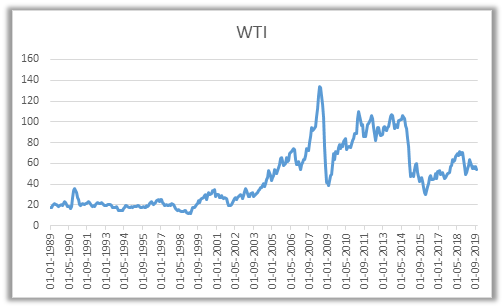
\includegraphics[width=0.4\paperwidth]{images/WTIPRICE.png}}
	\caption[Oil Price]{Crude WTI Price Series (US\$ / barrel)}
    \label{fig:oilprice3}
\end{figure}

An inspection of the similar time-series price data for related crude products (gasoline, light oil, jet fuel and kerosene) show similar patterns in price evolution.

\begin{figure}[!h]
    \centering
	\noindent\makebox[\textwidth]{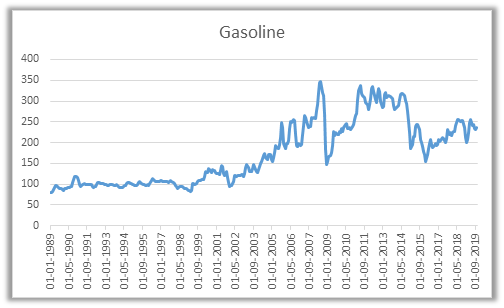
\includegraphics[width=0.4\paperwidth]{images/GASOLIN.png}}
	\caption[Oil Price]{Gasoline Price Series (US\$ / gallon)}
    \label{fig:oilprice4}
\end{figure}

\begin{figure}[!h]
    \centering
	\noindent\makebox[\textwidth]{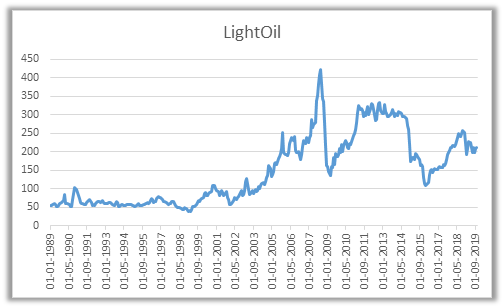
\includegraphics[width=0.4\paperwidth]{images/LIGHTOIL.png}}
	\caption[Oil Price]{Light Oil Price Series (US\$ / gallon)}
    \label{fig:oilprice5}
\end{figure}

\begin{figure}[!h]
    \centering
	\noindent\makebox[\textwidth]{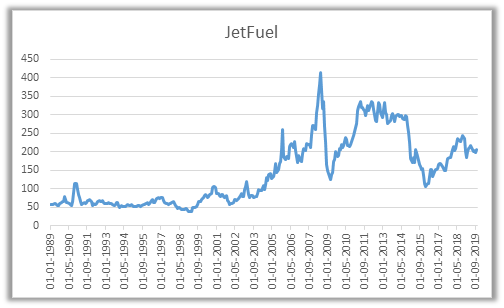
\includegraphics[width=0.4\paperwidth]{images/JETFUEL.png}}
	\caption[Oil Price]{Jet Oil Price Series (US\$ / gallon)}
    \label{fig:oilprice6}
\end{figure}

\begin{figure}[!h]
    \centering
	\noindent\makebox[\textwidth]{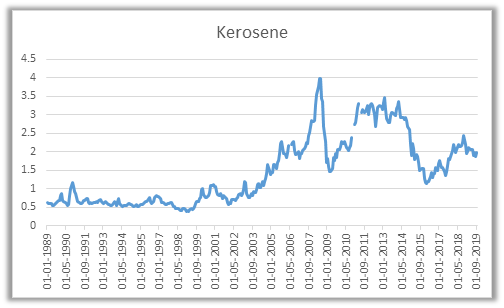
\includegraphics[width=0.4\paperwidth]{images/KEROSENE.png}}
	\caption[Oil Price]{Kerosene Price Series (US\$ / gallon)}
    \label{fig:oilprice7}
\end{figure}


\subsection{Exploratory Data Analysis – Q-Q Plot}
A Q-Q plot (Quantile-Quantile plot) is a visual tool used to check how much a set of data aligns with a theoretical distribution such as a Normal or Exponential distribution. It helps us inspect at a glance how two sets of data compare with each other from a distribution perspective. It is a scatterplot diagram generated by plotting two sets of data against each other. If the quantiles from both sets come from the same distribution, a nearly straight line is formed with a positive slope.\cite{cla2015}
The Q-Q plot for WTI crude oil is shown below.
\begin{figure}[!ht]
    \centering
	\noindent\makebox[\textwidth]{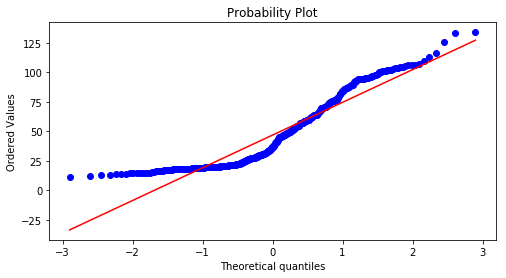
\includegraphics[width=0.6\paperwidth]{images/QQPLOT.png}}
	\caption[Oil Price]{QQ analysis of WTI Oil – QQ Plot}
    \label{fig:oilprice8}
\end{figure}
In the figure above, the red line represents theoretical normal distribution. If the WTI prices were perfectly normal in distribution, all the quantiles will lie on the red line. As seen above, the prices are roughly straight in nature suggesting a measure of normal distribution. It is also noted that a portion of the data is skewed right with a left-side distribution on the tail end. Otherwise, a good portion of the quantiles lie on the theoretical red line.
%Sets the bibliography style to UNSRT and imports the 
%bibliography file "samples.bib".
\section{Python Code for price Analysis}
\lstset{language=Python}
Required library need to be imported for execution of python code
\begin{lstlisting}
Python required following libraries to be imported.
import pandas as pd
from matplotlib import pyplot as plt
from scipy import stats
import statsmodels.api as sm
import seaborn as sns
from pandas.plotting import autocorrelation_plot
from statsmodels.tsa.arima_model import ARIMA
from sklearn.metrics import mean_squared_error
from sklearn.model_selection import train_test_split
\end{lstlisting}
Python version used is 3.*

We have data in the form of csv files. All csv files contain data from 1989 to 2019.
Csv files have two columns first is time series (monthly) and second commodity price.\\

Date,WTI\\
1989-01-01,18.02\\
1989-02-01,17.94\\
1989-03-01,19.48\\

\subsection{Read CSV data file}
\begin{lstlisting}
def readData(csvFile):
    data = pd.read_csv(csvFile, index_='Date', parse_dates=True)
    return data
\end{lstlisting}
This function reads data from csv file and returns dataframe having date as index.
\subsection{Plots commodity price with respect to time}
\begin{lstlisting}
def priceTrend(data):
    data.plot(figsize=(10,5), linewidth=1)
    plt.show()
\end{lstlisting}

\subsection{Calculate Variance of a datframe column}
\begin{lstlisting}
def getVAR(data, col):
    return data[col].var()
\end{lstlisting}

\subsection{Calculate Mean of a datframe column}
\begin{lstlisting}
def getMean(data, col):
    return data[col].mean()
\end{lstlisting}



\subsection{Plot distribution of data}
\begin{lstlisting}
def drawNormal(data, col):
    sns.distplot(data[col], hist = False, kde = True,
                 kde_kws = {'shade': True, 'linewidth': 3}, 
                  label = col)
    plt.ylabel('Density')
    plt.title('Density Plot')
    plt.show()
\end{lstlisting}

\subsection{skewness, kurtosis of column data }
\begin{lstlisting}
def getSkewAndKurt(data, col):
    mean   = data[col].mean()
    median = data[col].median()
    mode   = data[col].mode()
    skewness = data[col].skew()
    kurtosis = data[col].kurt()
    
    print('Mean = {}'.format(mean))
    print('Median = {}'.format(median))
    print('Mode = ', mode[0])
    print('Skewness = ', skewness)
    print('Kurtosis = ', kurtosis)
    
    plt.figure(figsize=(10, 5))
    plt.hist(data[col], bins=10, color='grey')
    plt.axvline(mean,color='red',label='Mean')
    plt.axvline(median,color='yellow',label='Median')
    plt.axvline(mode[0],color='green',label='Mode')
    plt.xlabel('Price')
    plt.ylabel('Frequency')
    plt.legend()
    plt.show()
    return skewness,kurtosis
\end{lstlisting}

\subsection{Plot Auto Co-relation of data}
\begin{lstlisting}
def drawAutoCorr(df, col):
    autocorrelation_plot(df[col])
    plt.show()
\end{lstlisting}

\subsection{Arima Model Fit Analysis}
\begin{lstlisting}
def arimaModelFitAnalysis(data, col):
    # fit model
    model = ARIMA(data[col], order=(5,1,0))
    model_fit = model.fit(disp=0)
    print(model_fit.summary())
    
    # plot residual erros
    residuals = pd.DataFrame(model_fit.resid)
    residuals.plot()
    residuals.plot(kind='kde')
    plt.show()
    print(residuals.describe())
\end{lstlisting}

\subsection{Arima Model Rolling Forcast}
\begin{lstlisting}
def arimaModelRollingForCast(data, col):
    X = data[col]
    size = int(len(X) * 0.66)
    train, test = X[0:size], X[size:len(X)]
    history = [x for x in train]
    predictions = []
    
    
    for t in range(len(test)):
        model = ARIMA(history, order=(5,1,0))
        model_fit = model.fit(disp=0)
        output = model_fit.forecast()
        yhat = output[0]
        predictions.append(yhat[0])
        obs = test[t]
        history.append(obs)
        print('predicted=%f, expected=%f' % (yhat, obs))
        
    error = mean_squared_error(test, predictions)
    print('Test MSE: %.3f' % error)
    df = pd.DataFrame(columns={'Test'})
    df['Test'] = test
    df['Predictions'] = predictions 
    # plot
    print(df.head())
    df.plot()
    plt.show()
\end{lstlisting}

\subsection{OLS Model}
\begin{lstlisting}
def olsModel(X, Y, y_col):
    X_train, X_test, y_train, y_test = train_test_split(X, Y, test_size=0.25)
    sm.add_constant(X_train)
    model = sm.OLS(y_train, X_train)
    result = model.fit()
    yPredict = result.predict(X_test)
    df = pd.DataFrame()
    df[y_col] = y_test;
    df[y_col + '_Predict'] = yPredict
    print(result.summary())
    df.plot()
\end{lstlisting}
Find linear relation between two commodities, this function predicts and plot the relation.
\newpage
\bibliographystyle{unsrt}
\bibliography{sample}

\end{document}
